% !TEX program = xelatex
\documentclass[aspectratio=43]{beamer}
\usetheme{metropolis}
\usepackage{hyperref}
\urlstyle{same}
\usepackage[super]{nth}
\usepackage{minted}
\usepackage{seqsplit}
\usepackage{graphicx}

\setbeamercovered{invisible}

\title{Neobuffer: Cross-Process Channels in Rust}
\author{Bernardo Meurer}
\date{June \nth{28}, 2019}
\institute{Standard Cognition}

\begin{document}
\maketitle

\begin{frame}{whoami}
    \begin{columns}[T]
        \begin{column}{.5\textwidth}
            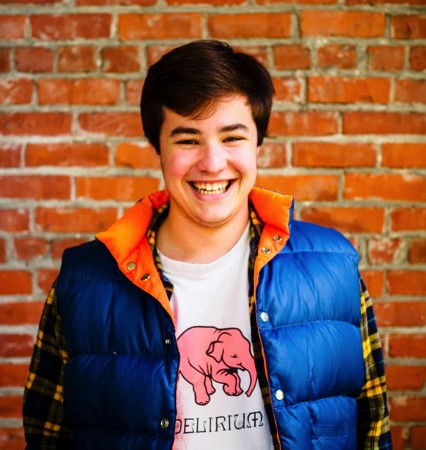
\includegraphics[width=\textwidth]{./imgs/bernardo-blue.jpg}
        \end{column}
        \begin{column}{.5\textwidth}
            \begin{block}{}
                \begin{itemize}
                    \item Bernardo Meurer (\texttt{\small{lovesegfault}})
                    \item Systems Engineer @ Standard Cognition \url{http://standard.ai}
                    \item \texttt{\small{bernardo@standard.ai}}
                    \item \url{http://lovesegfault.com/}
                \end{itemize}
            \end{block}
        \end{column}
    \end{columns}
\end{frame}

\begin{frame}{Outline}
    \begin{itemize}
        \item Motivation
        \item Requirements
        \item Alternatives
        \item Neobuffer
            \begin{itemize}
                \item Components
                \item Ringbuffer
                \item Sink
                \item Source
                \item Quirks
                \item Results
                \item Future work
            \end{itemize}
        \item Questions
    \end{itemize}
\end{frame}

\begin{frame}{whoarewe(?!)}
    \begin{columns}[T]
        \begin{column}{.5\textwidth}
            \begin{itemize}
                \item Standard Cognition
                \item SF + Tokyo
                \item Autonomous Checkout
                \item Python + Rust
                \item Many interesting problems to solve
                \item We're hiring!
            \end{itemize}
        \end{column}
        \begin{column}{.5\textwidth}
            
\includegraphics[width=\textwidth]{./imgs/sc-logo.png}
        \end{column}
    \end{columns}
\end{frame}

\begin{frame}<1>[label=motivation]{Motivation}
    \begin{itemize}
        \item<1-> We deal with a many cameras.
        \item<2-> We do experiments very frequently.
        \item<3-> How to multiplex the video streams?
        \item<4-> How to unify the API for controlling distinct cameras?
    \end{itemize}
\end{frame}
\begin{frame}{Motivation}
    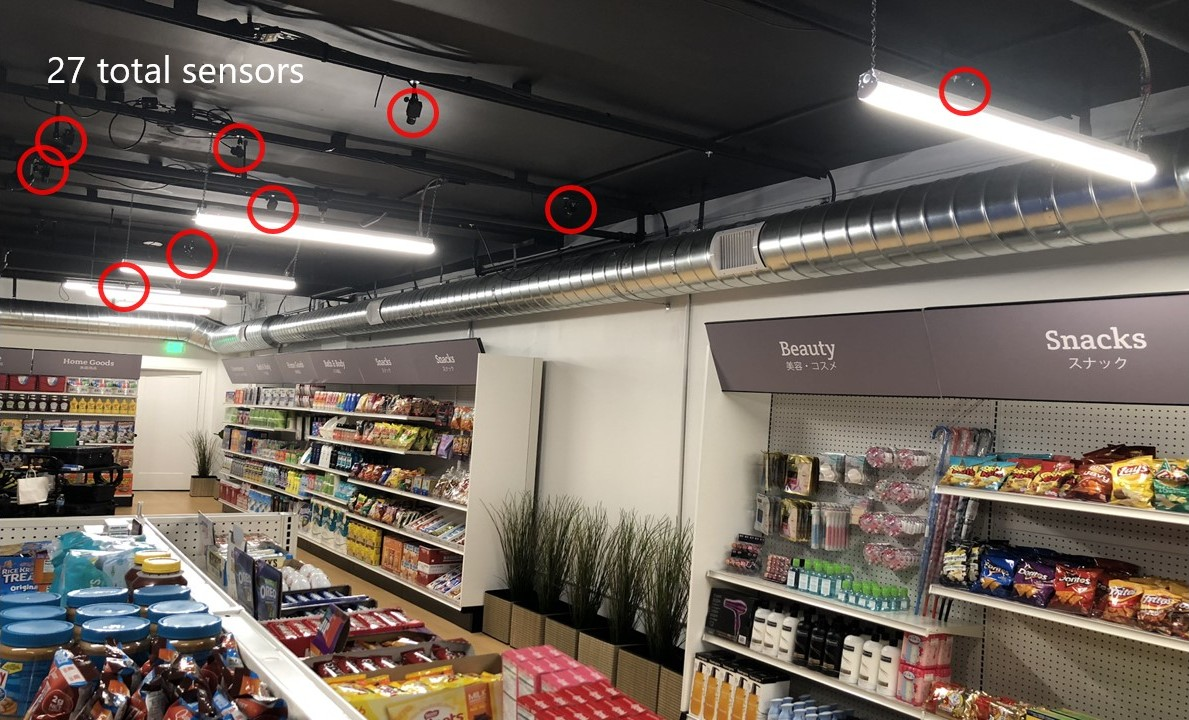
\includegraphics[width=\textwidth]{./imgs/cameras.jpg}
\end{frame}
\againframe<2>{motivation}
\begin{frame}{Motivation}
    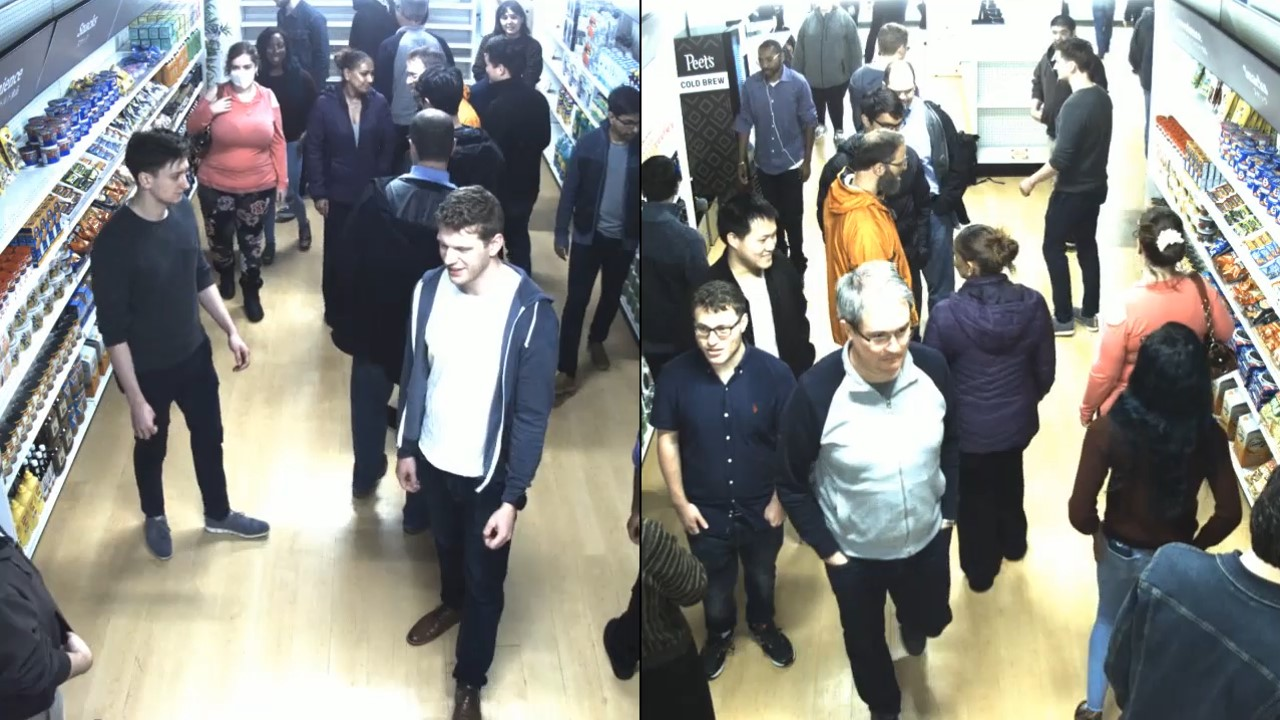
\includegraphics[width=\textwidth]{./imgs/experiment.jpg}
\end{frame}
\againframe<3->{motivation}

\begin{frame}<1-5>[label=sensord]{Sensord/Camd}
    \begin{itemize}
        \item<1-> We still haven't quite decided on a name...
        \item<2-> Camera daemon
        \item<3-> Clients use ZMQ to communicate with it
        \item<4-> Has client libs for Rust, and Python (PyO3)
        \item<5-> Reasonably large Rust project
        \item<6-> A small part of a huge system
        \item<7-> One challenge was clear from inception...
    \end{itemize}
\end{frame}
\begin{frame}[fragile]
    \frametitle{Sensord/Camd}
    \centering
    \begin{minted}[fontsize=\tiny]{text}
$ tokei ./sensord
-------------------------------------------------------------------------------
 Language            Files        Lines         Code     Comments       Blanks
-------------------------------------------------------------------------------
 C Header                2            4            4            0            0
 GLSL                    2           63           54            1            8
 Markdown                1           29           29            0            0
 Nix                     1           44           34            0           10
 Python                  1           28           17            4            7
 Rust                   47         9391         7457          880         1054
 Plain Text              1           13           13            0            0
 TOML                   14          274          240            0           34
-------------------------------------------------------------------------------
 Total                  69         9846         7848          885         1113
-------------------------------------------------------------------------------
    \end{minted}
\end{frame}
\againframe<6>{sensord}
\begin{frame}{Sensord/Camd}
    \centering
    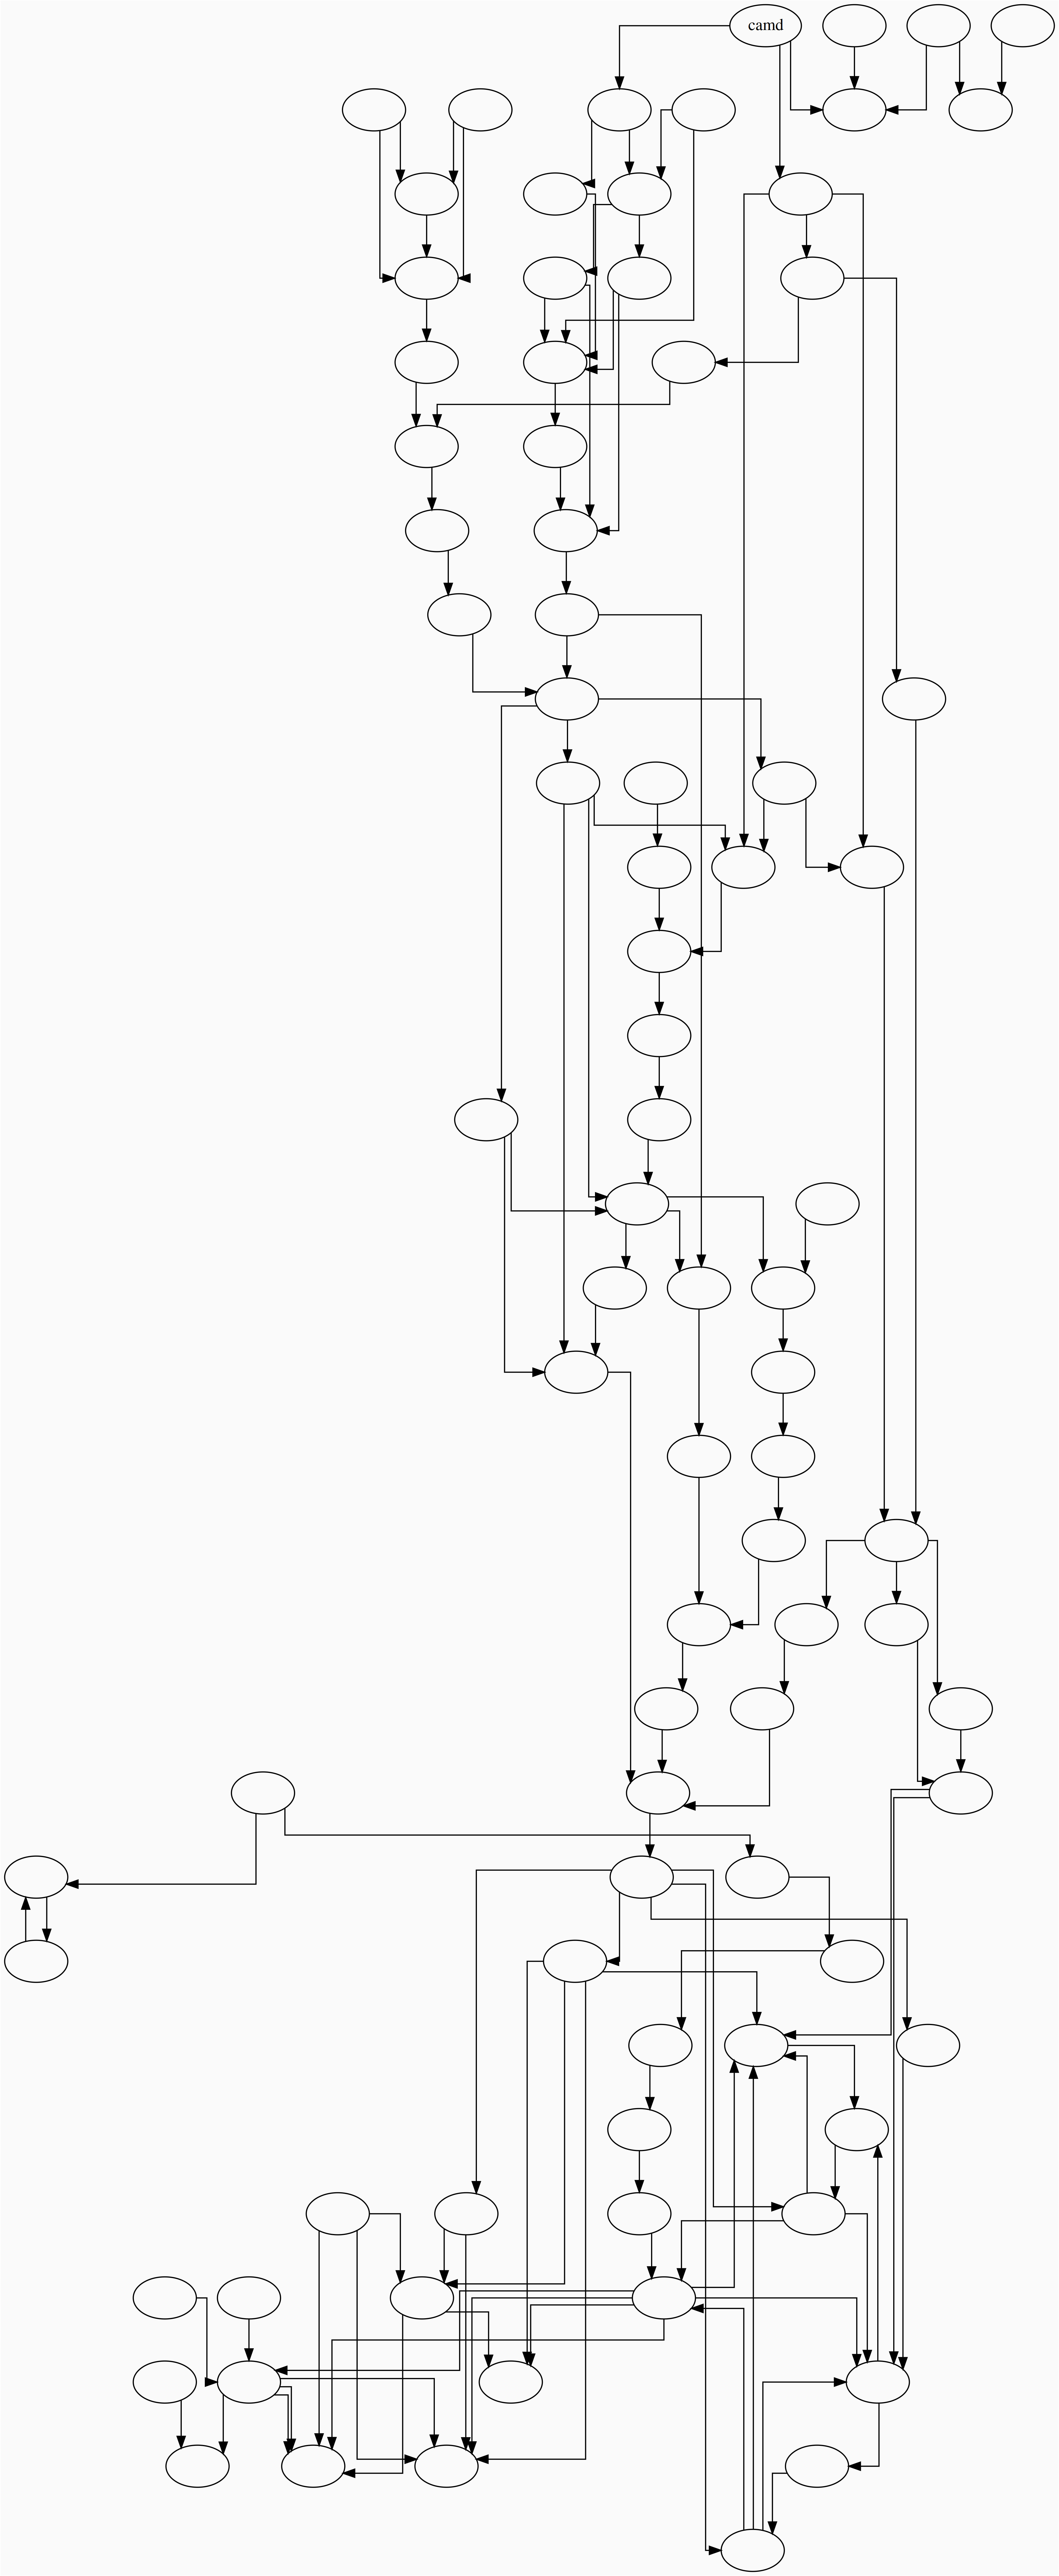
\includegraphics[height=8cm]{./imgs/camd-huge.jpg}
\end{frame}
\againframe<7->{sensord}

\begin{frame}{Sensord/Camd}
    \centering
    \begin{Large}
        How to connect \texttt{camd} to the client processes?
    \end{Large}
\end{frame}

\begin{frame}<1-3>[label=requirements]{Channel X: Requirements}
    \begin{itemize}
        \item<1-> Fast
        \item<2-> Lock-Free
        \item<3-> Flexible
        \item<4-> Cross-thread
        \item<5-> Cross-process
        \item<6-> Safe
        \item<7-> Multi-consumer
    \end{itemize}
\end{frame}
\begin{frame}{Channel X: Requirements}
    \centering
    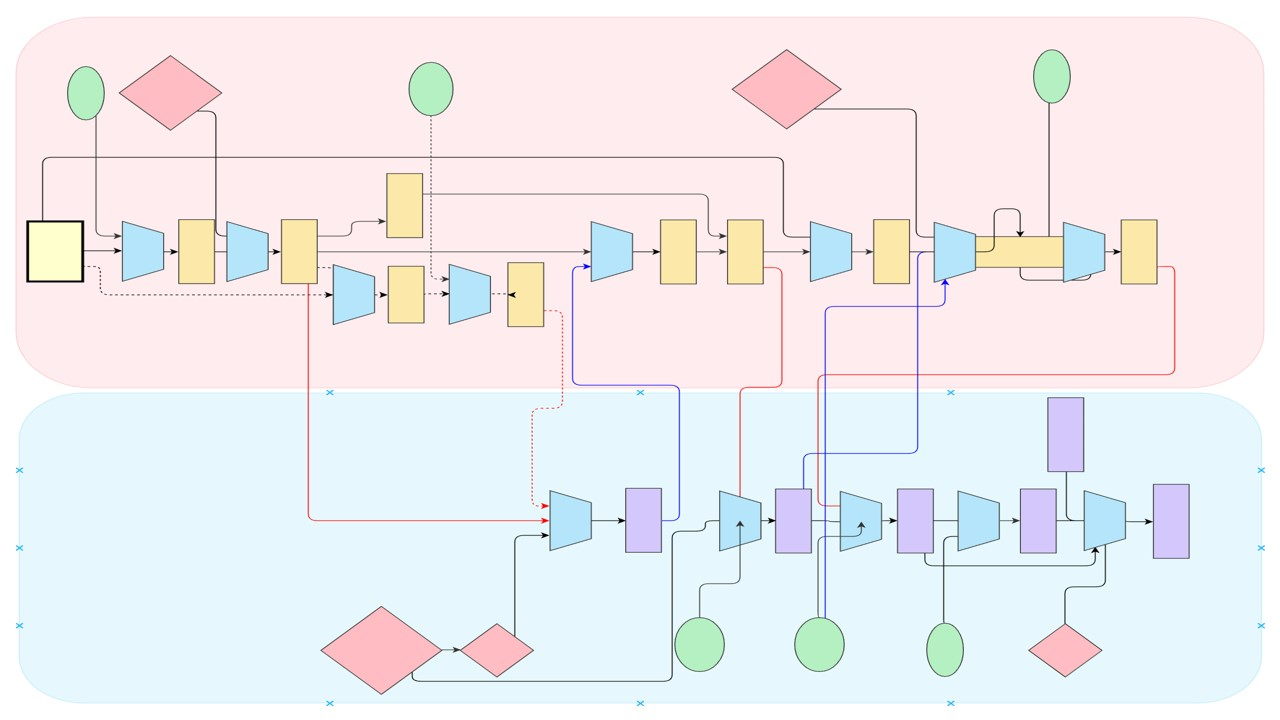
\includegraphics[width=\textwidth]{./imgs/system-graph.jpg}
\end{frame}
\againframe<4->{requirements}

\begin{frame}{Channel X: Who could it be?}
    \begin{columns}[T]
        \begin{column}{.5\textwidth}
            \begin{itemize}
                \item<1-> stdlib channels?
                \item<2-> \texttt{crossbeam}?
                \item<3-> \texttt{rb}?
                \item<4-> \texttt{ringbuf}?
            \end{itemize}
        \end{column}
        \begin{column}{.5\textwidth}
            
\includegraphics[width=\textwidth]{./imgs/who-is-channel.jpg}
        \end{column}
    \end{columns}
\end{frame}

\begin{frame}{Channel X: Neobuffer}
    \centering
    
\includegraphics[width=\textwidth]{./imgs/neobuffer.jpg}
\end{frame}

\begin{frame}{Neobuffer}
    \begin{itemize}
        \item Written from scratch
        \item 100\% Rust
        \item Collaboration with \texttt{ekleog} (Leo Gaspard) and
            \texttt{nagisa} (Simonas Kaslauskas)
        \item Based on discussions with \texttt{eddyb} and \texttt{amanieu}
    \end{itemize}
\end{frame}

\begin{frame}{Neobuffer: Components}
    \begin{itemize}
        \item<1-> Common traits for process-level \texttt{Sync} and
            \texttt{Send}
            \begin{itemize}
                \item \texttt{interprocess-traits} --- \texttt{ProcSync} and
                    \texttt{ProcSend}
                \item \url{github.com/standard-ai/interprocess-traits}
            \end{itemize}
        \item<2-> Shared memory for cross-process data sharing
            \begin{itemize}
                \item \texttt{shmem} --- An ergonomic wrapper around shared
                    memory for Rust
                \item \url{github.com/standard-ai/shmem}
            \end{itemize}
        \item<3-> Unix Domain Sockets for sending file descriptors across
            processes
            \begin{itemize}
                \item \texttt{sendfd} --- Utility crate that simplifies
                    \texttt{fd} sharing.
                \item \url{github.com/standard-ai/sendfd}
            \end{itemize}
        \item<4-> Ringbuffer for the underlying data structure
            \begin{itemize}
                \item Atomics for the indexes
                \item Careful application of memory orderings to guarantee
                    consistency
                \item Safe wrap around
                \item \url{github.com/standard-ai/neobuffer}
            \end{itemize}
    \end{itemize}
\end{frame}

\begin{frame}[fragile]{Neobuffer: \underline{Ringbuffer}, Sink, and Source}
    \begin{minted}[fontsize=\tiny]{rust}
/// A shared-memory ring buffer that contains items of type `T`, has one writer
/// and `NbReaders` readers that each read all the items the writer writes.
pub struct RingBuffer<T, NbReaders> {
    /// The shared memory region
    data: Shared<c_void>,

    /// The maximum number of elements this ring buffer can contain at a time.
    size: u64,

    /// Whether the one writer of this ring buffer has already been given out.
    writer_given: AtomicBool,

    /// The number of readers that have already been given out.
    readers_given: AtomicUsize,

    /// Phantom argument to keep type arguments alive.
    phantom: PhantomData<(T, NbReaders)>,
}
    \end{minted}
\end{frame}

\begin{frame}<1-3>[label=ringbuffer]{Neobuffer: \underline{Ringbuffer}, Sink, and Source}
    \begin{itemize}
        \item<1-> \texttt{Shared<T>} just means \texttt{T} is in shared memory
        \item<2-> \texttt{Shared<c\_void>} is a special case for data not sized
        \item<3-> But what exactly is in \texttt{Shared<c\_void>}?
        \item<4-> $M$ is the Ringbuffer metadata, and the magic smoke of
            Neobuffer
    \end{itemize}
\end{frame}

\begin{frame}[fragile]{Neobuffer: \underline{Ringbuffer}, Sink, and Source}
    \centering
    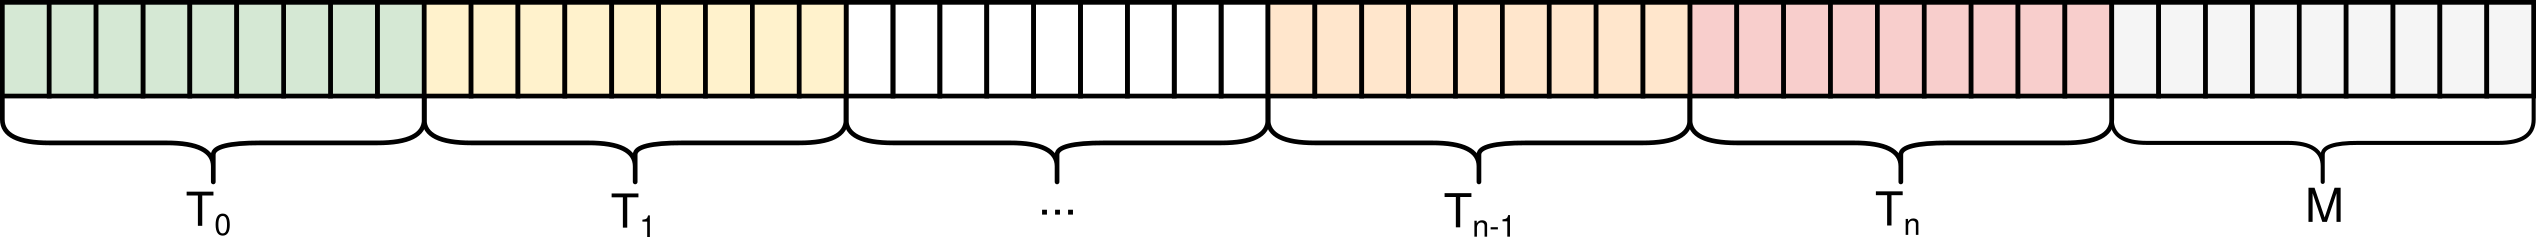
\includegraphics[width=\textwidth]{./imgs/neobuffer_layout.png}
\end{frame}

\againframe<4->{ringbuffer}

\begin{frame}[fragile]{Neobuffer: \underline{Ringbuffer}, Sink, and Source}
    \begin{minted}[fontsize=\tiny]{rust}
/// The metadata for the data stored in the `Shared`.
///
/// The actual data in the ringbuffer precedes this metadata, so that it can be
/// page-aligned. Elements between the minimal element of `reader_steps` and
/// `writer_step` (modulo `Size`) are the only initialized ones. The safety of
/// this relies on the fact that things in a `Shared` are guaranteed to not be
/// dropped, and to the dropping operations being manually handled.
#[repr(C)]
struct Metadata {
    /// Number of readers allocated in the metadata area (following this struct).
    ///
    /// This is immutable.
    reader_count: usize,

    /// The number of items that have ever been written. Monotonically
    /// increasing. `u64` is used here because `u32` might not be enough to
    /// handle a reasonable number of ring buffer additions.  However, all uses
    /// that are bounded by `Size` can safely assume it fits in `usize`.
    writer_step: AtomicU64,

    /// The number of outstanding references to this shared memory region.
    ///
    /// This knowledge is used to know when the remaining elements should be
    /// dropped.
    references: AtomicU64,
}
    \end{minted}
\end{frame}

\begin{frame}[fragile]{Neobuffer: \underline{Ringbuffer}, Sink, and Source}
    \begin{minted}[fontsize=\tiny]{rust}
impl<T, R> RingBuffer<T, R>
where
    // Ts are not created/inserted/shared here, so T does not need any bound here.
    R: Unsigned + NonZero,
{
    pub fn new(size: usize) -> Result<RingBuffer<T, R>, shmem::Error> {...}
    pub fn get_sink(&self) -> Result<Sink<T>, Error> {...}
    pub fn get_source(&self) -> Result<Source<T>, Error> {...}
}
    \end{minted}
\end{frame}

\begin{frame}[fragile]{Neobuffer: Ringbuffer, \underline{Sink}, and Source}
    \begin{minted}[fontsize=\tiny]{rust}
/// A sink that can send data into a `RingBuffer`.
pub struct Sink<T> {
    /// Shared pointer to the data.
    data: Shared<c_void>,

    /// Number of `T` that `data` has been allocated with.
    size: u64,

    /// Local copy of `data.writer_step`, that is not atomic for performance.
    writer_step: u64,

    /// Local helper that contains a value guaranteed to be lower to or equal
    /// to all values in `data.reader_steps`
    minimum_reader_step: Cell<u64>,

    /// Phantom argument to keep type arguments alive.
    phantom: PhantomData<T>,
}
    \end{minted}
\end{frame}

\begin{frame}[fragile]{Neobuffer: Ringbuffer, \underline{Sink}, and Source}
    \begin{minted}[fontsize=\tiny]{rust}
impl<T> Sink<T> {
    pub fn push(&mut self, item: T) -> nb::Result<(), Error> {...}
}
    \end{minted}
\end{frame}

\begin{frame}[fragile]{Neobuffer: Ringbuffer, Sink, and \underline{Source}}
    \begin{minted}[fontsize=\tiny]{rust}
/// A sink that can read data from a `RingBuffer`.
pub struct Source<T> {
    /// Shared pointer to the data.
    data: Shared<c_void>,

    /// Size of the ring buffer this is linked with.
    size: u64,

    /// Identifier of this reader in the `data.reader_steps` array.
    reader_id: usize,

    /// Local copy of `data.reader_steps[reader_id]`, for performance.
    reader_step: u64,

    /// Under-approximation of `data.writer_step`, local for performance.
    minimum_writer_step: Cell<u64>,

    /// Phantom argument to keep type arguments alive.
    phantom: PhantomData<T>,
}
    \end{minted}
\end{frame}

\begin{frame}[fragile]{Neobuffer: Ringbuffer, Sink, and \underline{Source}}
    \begin{minted}[fontsize=\tiny]{rust}
impl<T> Source<T> {
    pub fn available_size(&self) -> usize {...}

    /// Advance the reader discarding `n` lowest numbered elements in the buffer.
    ///
    /// This allows elements, which have been advanced past by all readers, to
    /// be overwritten.
    pub fn advance(&mut self, n: usize) -> nb::Result<(), Infallible> {...}

    /// Get a reference to `i`-th element stored in the buffer.
    ///
    /// Once the use of the reference is done, [`Source::advance`] must be
    /// called to advance the reader.
    pub fn get(&self, i: usize) -> nb::Result<&T, Infallible> {...}

    /// Handy combination of `get()` and `advance()`
    pub fn pop(&mut self) -> nb::Result<T, Infallible> {...}
}
    \end{minted}
\end{frame}

\begin{frame}{Neobuffer: Quirks}
    \begin{itemize}
        \item<1-> Consumption is local
        \item<2-> Relative indexing
        \item<3-> Only works on Linux
        \item<4-> You have to be surgically careful with atomic orderings
    \end{itemize}
\end{frame}

\begin{frame}[fragile]{Neobuffer: Results}
    \begin{minted}[fontsize=\tiny]{text}
one_writer_many_batching_readers_big   ... 10,693,940 ns/iter (+/- 931,225) = 1568 MB/s
one_writer_many_batching_readers_huge  ... 2,207,889 ns/iter (+/- 370,206) = 30395 MB/s
one_writer_many_batching_readers_small ... 9,169,666 ns/iter (+/- 411,746) = 7 MB/s
one_writer_many_readers_big            ... 7,919,200 ns/iter (+/- 584,713) = 2118 MB/s
one_writer_many_readers_huge           ... 2,219,540 ns/iter (+/- 186,404) = 30235 MB/s
one_writer_many_readers_small          ... 6,706,252 ns/iter (+/- 480,979) = 9 MB/s
one_writer_one_batching_reader_big     ... 3,522,033 ns/iter (+/- 18,138) = 4763 MB/s
one_writer_one_batching_reader_huge    ... 2,188,906 ns/iter (+/- 19,540) = 30658 MB/s
one_writer_one_batching_reader_small   ... 3,369,997 ns/iter (+/- 314,502) = 19 MB/s
one_writer_one_reader_big              ... 5,138,619 ns/iter (+/- 263,518) = 3264 MB/s
one_writer_one_reader_huge             ... 2,196,294 ns/iter (+/- 31,967) = 30555 MB/s
one_writer_one_reader_small            ... 3,213,515 ns/iter (+/- 360,083) = 20 MB/s
one_writer_two_batching_readers_big    ... 5,827,360 ns/iter (+/- 160,344) = 2879 MB/s
one_writer_two_batching_readers_huge   ... 2,201,807 ns/iter (+/- 14,876) = 30478 MB/s
one_writer_two_batching_readers_small  ... 4,877,466 ns/iter (+/- 184,255) = 13 MB/s
one_writer_two_readers_big             ... 5,310,644 ns/iter (+/- 149,770) = 3159 MB/s
one_writer_two_readers_huge            ... 2,195,695 ns/iter (+/- 91,573) = 30563 MB/s
one_writer_two_readers_small           ... 4,028,670 ns/iter (+/- 403,310) = 16 MB/s
    \end{minted}
\end{frame}

\begin{frame}{Neobuffer: Results}
    Assuming 4 parallel readers and a buffer size of 8:
    \begin{itemize}
        \item<1-> ~7 Mpps (1 byte packets)
            \begin{itemize}
                \item ~50Mpps with a buffer size of 2048
            \end{itemize}
        \item<2-> ~300 Gbps (2MB packets)
    \end{itemize}
\end{frame}

\begin{frame}{Neobuffer: Future work}
    \begin{itemize}
        \item<1-> Improve ergonomics around failure cases
        \item<2-> Split pushing into allocate + commit (remove a copy/clone)
        \item<3-> Swappable backend
        \item<4-> MPMC
        \item<5-> Futures
        \item<6-> Global consumption
    \end{itemize}
\end{frame}

\begin{frame}{Summary}
    \begin{itemize}
        \item<1-> Lock-free, fast, cross-process channel
        \item<2-> Ringbuffer in shared memory
        \item<3-> Public supporting libraries
        \item<4-> Atomics to manage read/write indexes
        \item<5-> Safe interface for cross-process communication
    \end{itemize}
\end{frame}


\begin{frame}{Questions?}
    \centering
    \Huge{There will be no questions}\\
    \centering
    \Large{Are there any questions?}
\end{frame}
\begin{frame}{Made with Free Software}
    This presentation was made using Free (as in Freedom) and Open Source
    software:
    \begin{itemize}
        \item Vim
        \item \LaTeX{} + Beamer + \texttt{metropolis}
        \item Graphviz
        \item Inkscape
        \item Some dude on Fiverr
    \end{itemize}
\end{frame}
\end{document}
